\documentclass[a4paper, 12pt, one column]{article}

%% Language and font encodings. This says how to do hyphenation on end of lines.
\usepackage[english]{babel}
\usepackage[utf8x]{inputenc}
\usepackage[T1]{fontenc}
\usepackage{aas_macros}

%% Sets page size and margins. You can edit this to your liking
\usepackage[top=1.3cm, bottom=2.0cm, outer=2.5cm, inner=2.5cm, heightrounded,
marginparwidth=1.5cm, marginparsep=0.4cm, margin=2.5cm]{geometry}

%% Useful packages
\usepackage{graphicx} %allows you to use jpg or png images. PDF is still recommended
\usepackage[colorlinks=False]{hyperref} % add links inside PDF files
\usepackage{amsmath}  % Math fonts
\usepackage{amsfonts} %
\usepackage{amssymb}  %
\usepackage{subfig}
\usepackage[table,xcdraw]{xcolor}
\usepackage{multirow}
\usepackage{spverbatim}
\usepackage{lineno}
\usepackage{array}
%% Citation package
\usepackage[]{natbib}
\bibliographystyle{unsrt}
% \setcitestyle{authoryear,open={(},close={)}}


\title{Introduction to \LaTeX \space and \texttt{GIT}}
\author{KM Mukut}

\begin{document}
\maketitle

\begin{abstract}

    \LaTeX is a document preparation system for high-quality typesetting used for medium-to-large technical or scientific documents, however,  it can be used for almost any form of publishing. It is technically not a word-processor, rather its main purpose is to make sure the appearance of the document is \textcolor{blue}{automatically} taken care of without the supervision of the author. 
    
    \vspace{0.3cm}

    \fcolorbox{red}{white} {
        \rotatebox{0}
            {
            \begin{minipage}{0.8\textwidth}
                \centering
               \LaTeX \space automatically makes your document beautiful and organized 
            \end{minipage}
            }
        }

\end{abstract}

\section{\LaTeX\space vs. Word processors}
\begin{linenumbers}

    
\begin{figure}[!httb]
    \centering
    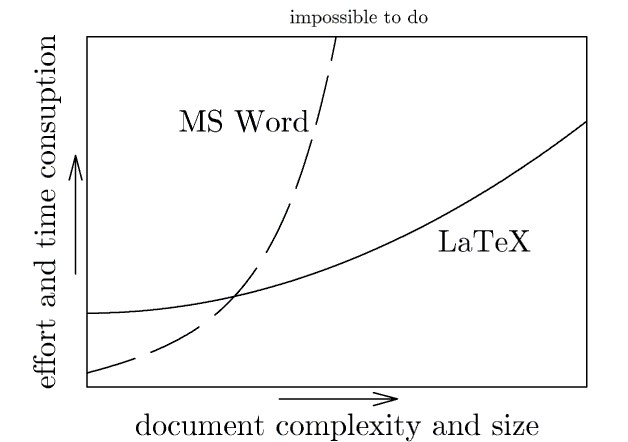
\includegraphics[width=0.6\linewidth]{wordvslatex.jpg}
    \caption{Word Processors vs. \LaTeX}
    \label{wordvslatex}
    \end{figure}
Using a word-processor (MS Word, LibreOffice,  Pages etc.) only makes sense while writing short documents and get the output quickly. For larger documents with many cross-references, equations,  figures and tables, \LaTeX \space makes things easier and faster. Fig. \ref{wordvslatex} is a nice demonstration to show the complexity and effort necessary for writing documents using MS Word and \LaTeX  \cite{BibEntry2020Apr}. All journals provide \LaTeX \space template for writing manuscripts in their specific formats. Since all the initial document set up is provided,  writing manuscripts using \LaTeX \space exceptionally easy and less time-consuming. Marquette university also have a \LaTeX \space template for Ph.D. and MS thesis, available at: \textcolor{blue}{\url{https://ctan.org/tex-archive/macros/latex/contrib/mugsthesis}}

\end{linenumbers}

\vspace{0.3cm}

\fcolorbox{red}{white} {
    \rotatebox{0}
        {
        \begin{minipage}{0.9\textwidth}
            \centering
           \LaTeX \space is well suited for writing complex documents with cross-references, equations, figures and tables efficiently. 
        \end{minipage}
        }
    }





\section{Writing Equations using \LaTeX}

    Managing equation in word processor is really challenging and time-consuming. Writing equations in \LaTeX \space is exceptionally easy and intuitive.  In \LaTeX , equations are easy to create and edit. Both PowerPoint and Word now have equation editors that allow for \LaTeX \space (see Fig. \ref{eqWord} ). 

    \begin{figure}[!httb]
        \centering
        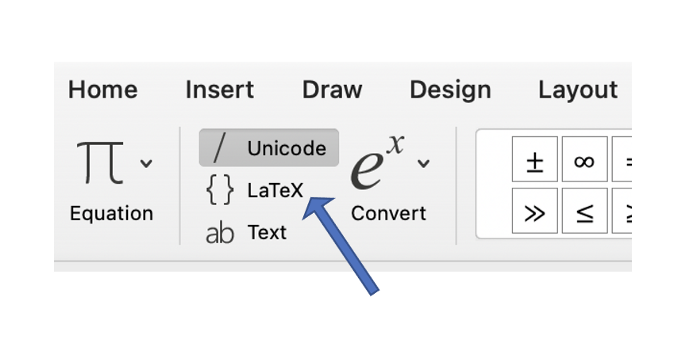
\includegraphics[width=0.6\linewidth]{eqWord.png}
        \caption{ \LaTeX \space style equation editor in PowerPoint}
        \label{eqWord}
        \end{figure}

    There are several methods for writing equation in \LaTeX, i.e. inline, aligned, equation, gathered etc. The basic \LaTeX markup for writing equations is shown in Fig. \ref{eqDemo}. 

    \begin{figure}[!httb]
        \centering
        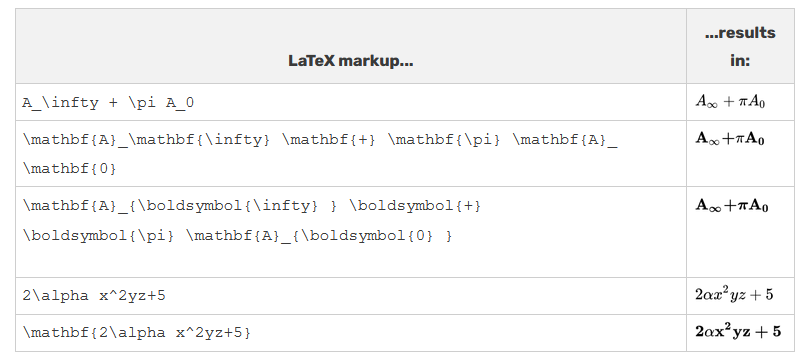
\includegraphics[width=0.8\linewidth]{eqDemo.png}
        \caption{ \LaTeX \space style equation markup example}
        \label{eqDemo}
        \end{figure}

    Equations can be written in line math such as $a^2+b^2=c^2$ . One can also give equations their own space (Equation \ref{sampleeq1}). The equations can be as complex as you want them to be ((Equation \ref{sampleeq2}))

   \begin{equation} 
   \gamma^2+\theta^2=\omega^2
   \label{sampleeq1}
   \end{equation}

   \begin{equation} 
    \mathcal{L}_{\mathcal{T}}(\vec{\lambda}) = \sum_{\mathbf{x},\mathbf{s}\in\mathcal{T}} \log P(\mathbf{x}|\mathbf{S}) - \sum_{i=1}^m \frac{\lambda_i^2}{2\sigma^2}
    \label{sampleeq2}
  \end{equation}
You can be really creative with how you want to present your equation sets (\ref{sampleeq3} and \ref{sampleeq4})
  \begin{align} 
    \label{sampleeq3}
    x&=y           &  w &=z              &  a&=b+c \nonumber \\
    2x&=-y         &  3w&=\frac{1}{2}z   &  a&=b\\
    -4 + 5x&=2+y   &  w+2&=-1+w          &  ab&=cb \nonumber
    \end{align}

    \begin{align}
        \label{sampleeq4}
        f(x_1, x_2, x_3) = & f_0 m_0 \vee f_1 m_1 \vee f_3 m_3 \vee \nonumber \\
          & \vee f_4 m_4 \vee f_5 m_5 \vee f_6 m_6 \vee f_7 m_7 \nonumber \\
        = & 0 m_0 \vee 1 m_1 \vee 0 m_3 \vee \\
          & \vee 1 m_4 \vee 0 m_5 \vee 0 m_6 \vee 1 m_7 \nonumber 
    \end{align}

    \vspace{0.3cm}

    \fcolorbox{red}{white} {
        \rotatebox{0}
            {
            \begin{minipage}{0.9\textwidth}
                \centering
            \LaTeX \space provides the fastest way to write complex mathematical equation with symbols, subscripts and superscripts
            \end{minipage}
            }
        }

\section{Building Tables with \LaTeX}

Building tables using \LaTeX is done using the ``Tabular'' environment.  If the table becomes large and complex, it gets tricky to manage. I usually use a website: \url{https://www.tablesgenerator.com/latex_tables} which is an excellent tool for generating \LaTeX \space code for large and complex tables. For demonstration, Table \ref{tb1} is generated using the abovementioned website as shown in Fig. \ref{tbDemo}. 

\begin{figure}[!httb]
    \centering
    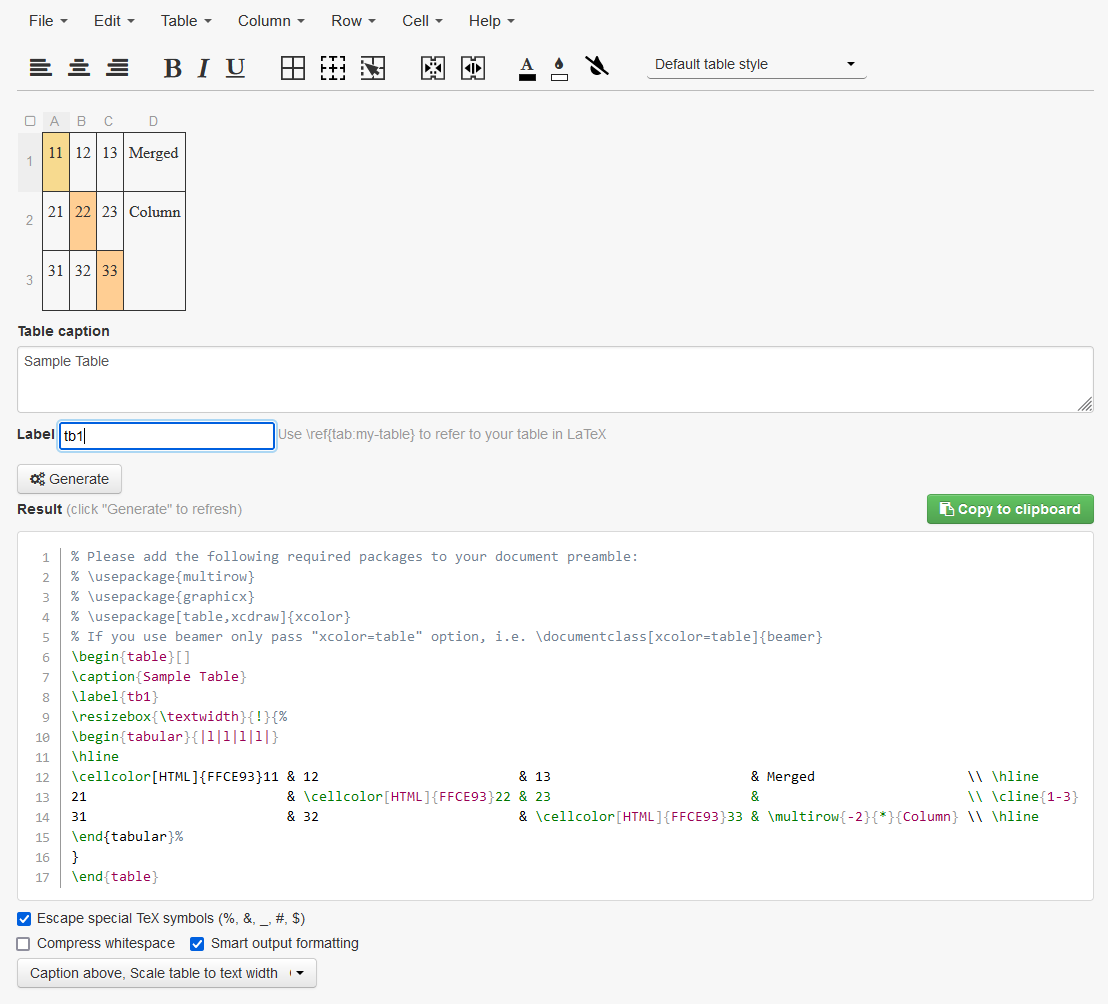
\includegraphics[width=0.9\linewidth]{Capture.PNG}
    \caption{ Demo of \LaTeX \space table generation}
    \label{tbDemo}
    \end{figure}

\begin{table}[!httb]
    \caption{A Sample Table}
    \label{tb1}
    \resizebox{\textwidth}{!}{%
    \begin{tabular}{|l|l|l|l|}
    \hline
    \cellcolor[HTML]{FFCE93}11 & 12                         & 13                         & Merged                   \\ \hline
    21                         & \cellcolor[HTML]{FFCE93}22 & 23                         &                          \\ \cline{1-3}
    31                         & 32                         & \cellcolor[HTML]{FFCE93}33 & \multirow{-2}{*}{Column} \\ \hline
    \end{tabular}%
    }
    \end{table}

\section{Citation Management in \LaTeX}

\LaTeX \space citation management is effortless. All the citations can be kept in a separate file (in this case \textcolor{blue}{``refs.bib''}) in bibtex format. Every time, a citation is required, we just write \textcolor{blue}{ \textbackslash cite\{key used in .bib file\}}. For example, Mukut et. al. \cite{Mukut2022Jul} or Claydon et al. \cite{Claydon17}. All the citations used in the document will be summarized at the end of the document. 

\section{List of Contents,  Figures and Tables}


\fcolorbox{red}{white} {
    \rotatebox{0}
        {
        \begin{minipage}{0.9\textwidth}
            \centering
        Creating list of Contents, Figures and Table is really easy in \LaTeX
        \end{minipage}
        }
    }
\tableofcontents
\listoffigures
\listoftables



\section{How can we use \LaTeX}
\LaTeX \space is an open-source tool which is freely available in all platforms. You can use any one of the following: 
\begin{enumerate}
    \item For Windows: \texttt{MiKTeX, proTeXt or Tex Live}
    \item For Linux: \texttt{Tex Live}
    \item For MacOS: \texttt{MacTex}
    \item From Online: \texttt{Papeeria, Overleaf, ShareLaTex, Datazar, and LaTeX base}
\end{enumerate}

\vspace{0.3cm}
\fcolorbox{red}{white} {
    \rotatebox{0}
        {
        \begin{minipage}{0.9\textwidth}
            \centering
        I personally use the offline version of \LaTeX \space alongside with a text editor called \textcolor{blue}{ \texttt{VSCode}}
        \end{minipage}
        }
    }

\section{A Short Introduction to \texttt{GIT}}

\texttt{GIT} is a version control system (VCS) for tracking changes in a project. This is a widely used tool for managing large-scale programs like Linux kernel, but it can also be used for smaller scale projects like your own programming projects, homework, assignments, papers, or thesis. \texttt{GIT} is freely available in all platform. There are several online platforms which let you maintain a cloud repository for better collaboration and safety (\texttt{GitHub, GitLab etc.}). \texttt{GitHub} is the most popular of them all. 

\subsection{\texttt{GIT} Workflow I Use for \LaTeX}
\begin{enumerate}
    \item Set up the working directory as a \texttt{GIT} repository (enable version control)
    \item Make a cloud version of the repository using your favorite \texttt{GIT} server, i.e. \texttt{GitLab}, \texttt{GitHub} etc. 
    \item Maintain separate branches for the master version, and any collaboration. 
    \item Work on my computer on my specific branch and when done use the following command: \label{mine}
    \begin{spverbatim}
        git add <any new files that has been created>
        git commit -a -m <specific message for the new updates> 
            ==> This will update the current state of the branch
        git checkout <The main/master branch> 
            ==> go to the main/master branch
        git merge <the branch I am working in> 
            ==> update the main/master branch with my edits
        git push  
            ==> This will sync the cloud repository in GitHub or GitLab

    \end{spverbatim}

    \item My collaborator will do the following: \label{his}
    \begin{spverbatim}
        git pull 
            ==> get the updates from the cloud repository
        git merge <his/her working branch>
            ==> sync the main/master branch to their working branch

        Edit/review the project, add comments, etc.     

        git add <any new files that has been created>
        git commit -a -m <specific message for the new updates> 
            ==> This will update the edits in their local repository
        git checkout <The main/master branch> 
            ==> go to the main/master branch
        git merge <the branch the collaborator is working in> 
            ==> update the main/master branch with the collaborator's edits
        git push  
            ==> This will sync the cloud repository in GitHub or GitLab
    \end{spverbatim}
    \item go back and forth between \ref{mine} and \ref{his} until the final version is ready. 
\end{enumerate}



\bibliography{refs}
\end{document}
